%%%%%%%%%%%%%%%%%%%%%%%%%%%%%%%%%%%%%%%%%%%%%%%%%%%
%
%  New template code for TAMU Theses and Dissertations starting Fall 2016.  
%
%
%  Author: Sean Zachary Roberson
%  Version 3.17.09
%  Last Updated: 9/21/2017
%
%%%%%%%%%%%%%%%%%%%%%%%%%%%%%%%%%%%%%%%%%%%%%%%%%%%
%%%%%%%%%%%%%%%%%%%%%%%%%%%%%%%%%%%%%%%%%%%%%%%%%%%%%%%%%%%%%%%%%%%%%%
%%                           TIME TO SOLUTION ESTIMATOR CHAPTER
%%%%%%%%%%%%%%%%%%%%%%%%%%%%%%%%%%%%%%%%%%%%%%%%%%%%%%%%%%%%%%%%%%%%%



\chapter{TIME TO SOLUTION ESTIMATOR \label{cha:tts}}

This chapter is for the time to solution estimator description.

\section{Method}
The detailed method description will go here.

\section{2D Verification}
The 2d verification results will go here.

\begin{figure}[H]
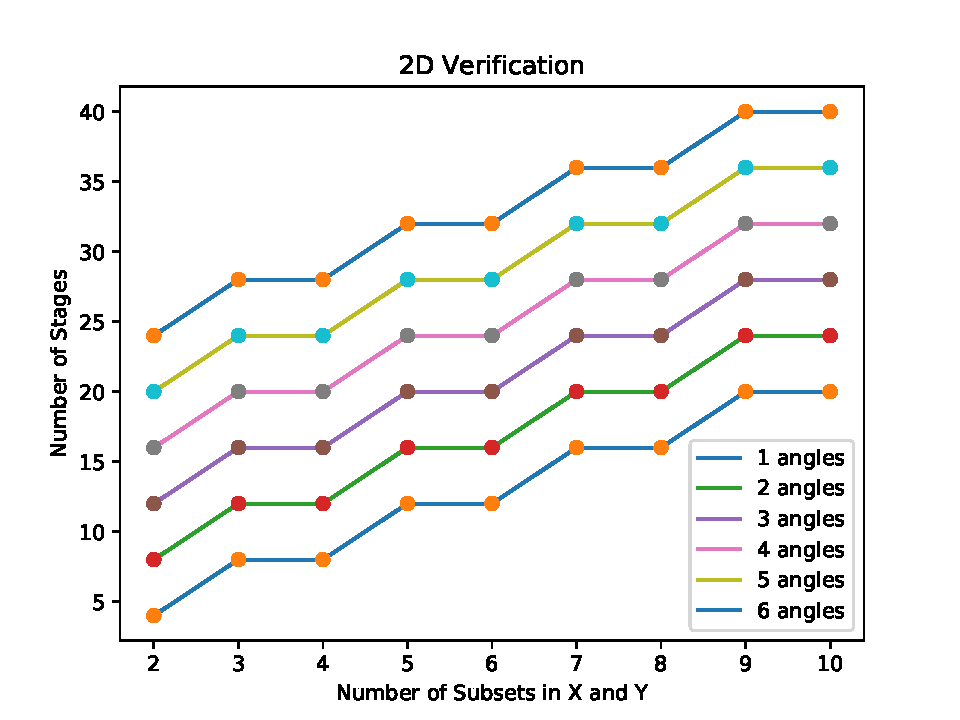
\includegraphics{../figures/regular_verification.pdf}
\caption{A 2D verification suite with regular partitions run from 2x2 to 10x10 subsets with each case being run from 1 to 6 angles per quadrant.}
\label{regular_verification}
\end{figure}

\begin{figure}[H]
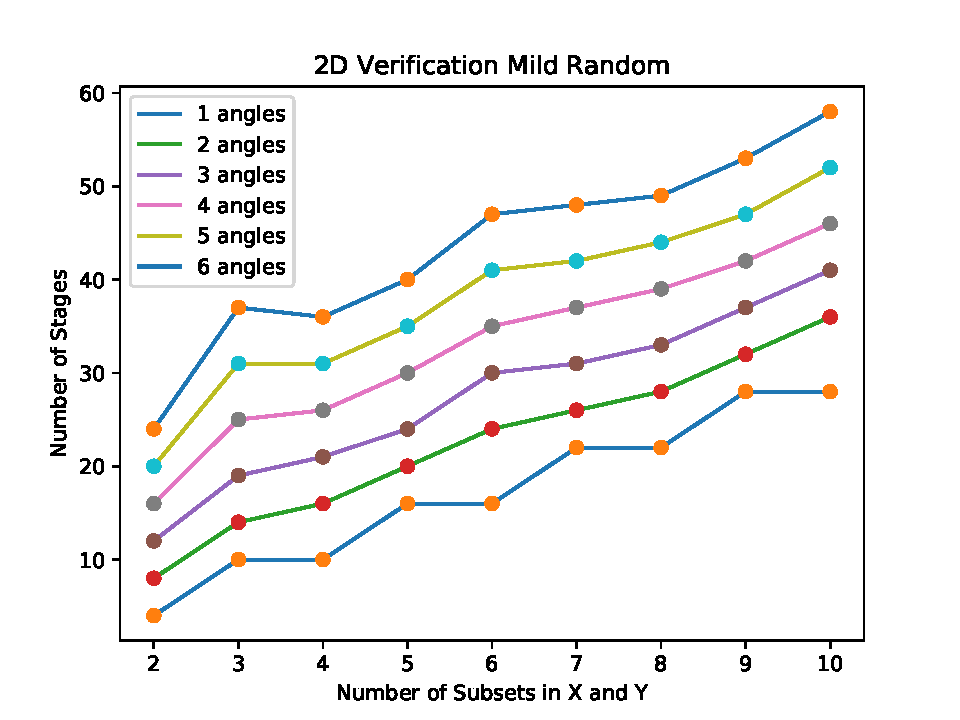
\includegraphics{../figures/mild_random_verification.pdf}
\caption{A 2D verification suite with mildly random partitions run from 2x2 to 10x10 subsets with each case being run from 1 to 6 angles per quadrant.}
\label{regular_verification}
\end{figure}

\begin{figure}[H]
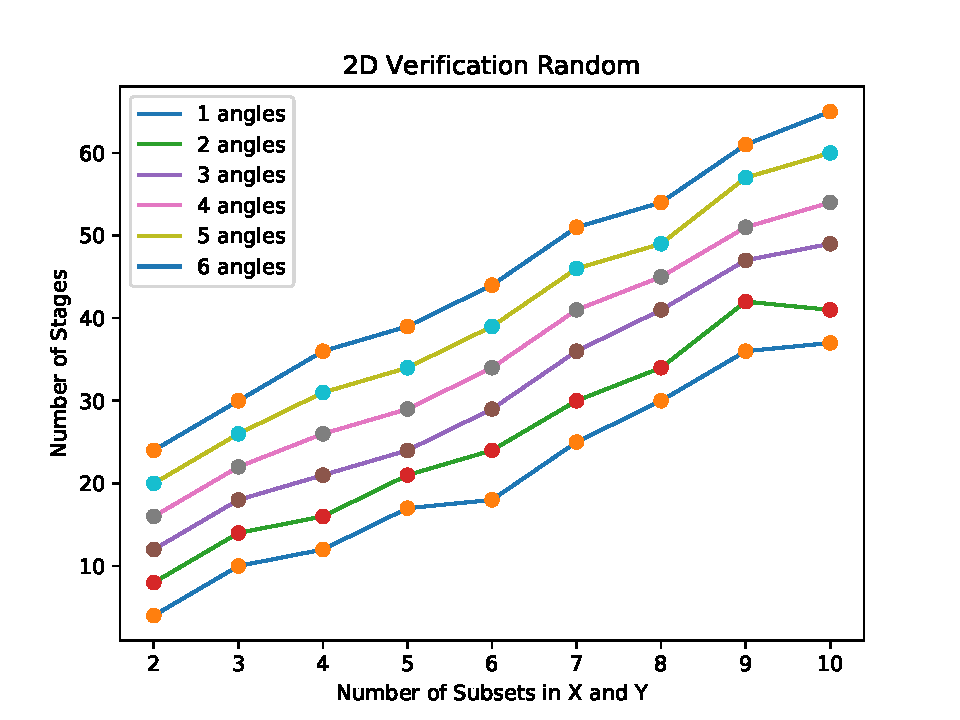
\includegraphics{../figures/random_verification.pdf}
\caption{A 2D verification suite with random partitions run from 2x2 to 10x10 subsets with each case being run from 1 to 6 angles per quadrant.}
\label{regular_verification}
\end{figure}

\begin{figure}[H]
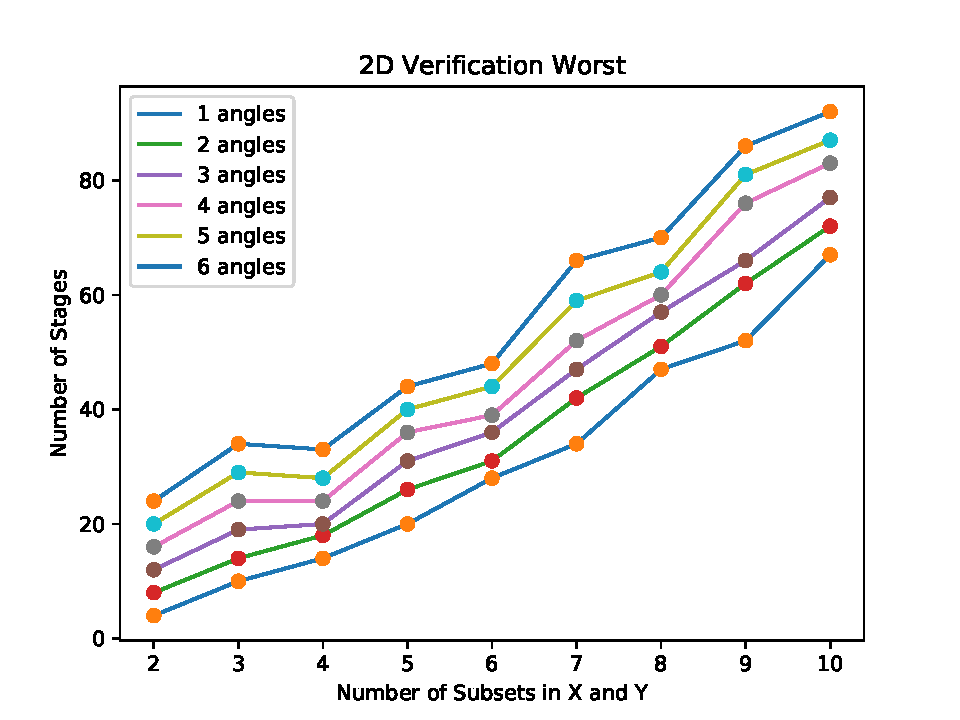
\includegraphics{../figures/worst_verification.pdf}
\caption{A 2D verification suite with probable worst-case partitions run from 2x2 to 10x10 subsets with each case being run from 1 to 6 angles per quadrant.}
\label{regular_verification}
\end{figure}

\section{3D Verification}

The 3d verification results will go here.
